\documentclass[titlepage]{article}
\usepackage{xeCJK}
\usepackage{fontspec}  
\usepackage{fancyhdr}  
\usepackage{indentfirst} 
%\usepackage[xetex]{hyperref}
%\usepackage{hyperref}
\usepackage{color}
\usepackage{listings}
\usepackage{xcolor}
\usepackage{graphicx}

\usepackage{paralist}
\usepackage[xetex,
            bookmarksnumbered,
            bookmarksopen,
            colorlinks,
%            urlbordercolor={111 111 111},
%            citecolor=blue,
            linkcolor=blue,
%            anchorcolor=blue,
            urlcolor=blue,
            ]{hyperref}
%\usepackage[CJKbookmarks]{hyperref}  

%\setlength{\parindent}{2em}
\addtolength{\hoffset}{-1cm}
\addtolength{\textwidth}{2cm}

\setCJKmainfont{STHeiti}
\setmainfont{Menlo} 
\begin{document}

%\lstset{numbers=left,
%numberstyle=\tiny,
%keywordstyle=\color{blue!70}, commentstyle=\color{red!50!green!50!blue!50},
%frame=shadowbox,
%rulesepcolor=\color{red!20!green!20!blue!20}
%}
\lstset{ 
frame=shadowbox, 
%numbers=left, 
%numberstyle=\tiny, 
escapeinside=``, 
xleftmargin=2em, 
xrightmargin=2em, 
aboveskip=1em,
rulesepcolor=\color{red!20!green!20!blue!20},
%rulesepcolor=\color{brown}
%keywordstyle=\color{blue!70}, 
%commentstyle=\color{red!50!green!50!blue!50}, 
keywordstyle=\color{blue}\bfseries,
commentstyle=\color{olive},
%directivestyle=\color{blue},
stringstyle=\color{purple},
%backgroundcolor=\color{gray},
%basicstyle=\tiny\ttfamily,
%basicstyle=\tiny,
%framerule=0pt,
breaklines=true,
}

\pagestyle{fancy}
\lhead{}
\lfoot{}
\cfoot{}
\rfoot{}
\renewcommand{\headrulewidth}{0.4pt}
\renewcommand{\footrulewidth}{0.4pt}

\title{个人简历} 
\author{金磊} 
\renewcommand{\today}{\number\year 年 \number\month 月 \number\day 日}
\date{\today} 
\maketitle

\setlength{\parindent}{2em} 
\addtolength{\parskip}{3pt}

%\pdfbookmark[2]{Bookmarktitle}{internallabel}
\renewcommand{\contentsname}{目录}
\setcounter{tocdepth}{2}
\tableofcontents 

\newpage
\section{基本情况}

\begin{tabular}{|l|l|}
\hline
姓名 & 金磊 \\
\hline
年龄 & 32 \\
\hline
出生年月 & 1982-02 \\
\hline
毕业院校 & 天津大学 \\
\hline
学历 & 通信系统工程硕士 \\
\hline 
出生地 & 天津 \\
\hline 
手机 & 13820788636 \\
\hline 
住址 & 北京昌平 \\
\hline 
婚姻状况 & 已婚 \\
\hline 
邮箱 & 125981281@qq.com \\
\hline 
github & \href{http:/www.github.com/jinleileiking?tab=repositories}{github.com/jinleileiking} \\
\hline
\end{tabular}



\section{工作经历}

\begin{tabular}{|l|l|l|}
\hline
2006-2007 & 华为3com实习 & 软件工程师 \\
\hline
2007-2014 & 	中兴天津研究 & 	软件工程师,系统工程师 \\
\hline
2014.3-2014.6 & 	AmpedRf  & 	高级嵌入式软件工程师 \\
             &  http://www.ampedrftech.com &                         \\
\hline
2014.6-至今 & 百度 & 高级研发工程师 \\
\hline
\end{tabular}

\section{教育经历}

\begin{tabular}{|l|l|l|l|l|}
\hline
2004-2007 & 天津大学  & 研究生 &  主修神经网络 & 毕业设计 \\
          & 通信工程  &        & 现代编码与调制&“基于ARM S3C44B0的\\
          &           &        & 通信网理论    & 嵌入式uCLinux下\\
          &           &        & 数字信号处理  &的温控湿热室”\\
\hline
2000-2004 & 南京理工大学  & 本科 &  通信信息系统 &  \\
\hline
\end{tabular}


\section{技能}

\subsection{工作技能}



\subsubsection{openwrt开发}

掌握的技能有

\begin{compactitem}
    \item nginx\_lua 
    \item lua\_resty\_memcache 
    \item nginx\_cache 
    \item memcache 
    \item lua\_memcache
    \item wormhole 
    \item http 
    \item spdy 
    \item 浏览加速
    \item firebug 
    \item linux tcp/ip协议栈
    \item netfilter
    \item openwrt的架构,make流程
    \item 将openwrt的一个opk移植到其他嵌入式设备上
    \item mongoose http server
    \item ubus system
    \item android zygote移植
    \item 软件包实时升级
    \item nf\_conntrack
    \item hack tcp/ip stack in linux kernel with the  netfilter
    \item anti-phishing
    \item linux kernel netlink
    \item linux kernel timer
    \item gdb 
    \item git 
    \item gerrit
    \item jenkins
    \item nginx\_cache hacking
    \item linux process management, keepalive.
    \item mqtt
    \item websocket
    \item 使用ruby进行测试
\end{compactitem}



\subsubsection{linux开发}

这一部分主要是在linux进行操作系统的编程, 驱动修改。

用过的cpu有:

\begin{compactitem}
    \item arm nxp lpc2138, 
    \item arm sumsumg s3c6410
    \item arm ti am335x
    \item arm ti am1808
\end{compactitem}

外设驱动,开发过

\begin{compactitem}
    \item 串口
    \item i2c
    \item spi
    \item usb
    \item eth
    \item rs485
    \item lcd
    \item dac
    \item adc
    \item 高频芯片(rc533 pn531)
    \item eeprom
    \item mmcsd
    \item wifi
    \item psam
\end{compactitem}

应用实现

\begin{compactitem}
    \item 网口的LLRP协议。
    \item 使用过sqlite数据库。
    \item 移植过ruby+sinatra小型嵌入式服务器。
    \item 熟练掌握uboot修改。
    \item 内核驱动修改
    \item 内核裁剪。
\end{compactitem}



\subsubsection{单片机开发}

这一部分主要是在IDE对CPU进行非linux操作系统的编程。

用过的cpu有:

\begin{compactitem}
    \item arm7的lpc2138,
    \item ti msp430
    \item freescale的cpu
    \item atmel
    \item energemicro的cpu等。
\end{compactitem}

开发方式都是IDE(Keil, IAR)+JTAG。

使用freeRTOS, 熟悉lwip协议栈。

外设驱动,开发过

\begin{compactitem}
    \item 串口
    \item i2c
    \item spi
    \item usb
    \item eth
    \item rs485
    \item lcd
    \item dac
    \item adc
    \item 高频芯片(rc533, pn531)
\end{compactitem}

应用开发过

\begin{compactitem}
    \item wifi协议栈
    \item 用arm实现过18000-6c协议
    \item EPCC1G2协议
    \item ISO7816协议
    \item 二义性协议
\end{compactitem}


\subsubsection{协议掌握}

熟练掌握各种协议,包括

\begin{compactitem}
    \item EPC C1G2
    \item 18000-6B/6C
    \item LLRP
    \item ATM
    \item X.25
    \item NFC
    \item eNFC
    \item PBOC
    \item 7816
    \item 14443
    \item ETC,二义性
    \item 802.11
\end{compactitem}


\subsection{其他技能}

\begin{compactitem}
    \item 能看懂硬件电路图,广泛阅读各种datasheet. 
    \item 熟练掌握 C\#.net winform编程
    \item 熟练掌握 ruby gtk编程
    \item 熟练掌握java swing编程 
    \item 掌握ruby on rails.
    \item 熟练掌握lua,写过几个WOW插件。
    \item 使用VIM+ GENTOO
    \item 使用git
    \item 用lua写了一个chrome插件,报告天津PM2.5值: https://chrome.google.com/webstore/detail/tjpm25/ilnkggadnkibhpmhedlgbdebkbndankb
    \item 使用Markdown。
    \item 使用latex。没错,这篇简历就是用latex写的。
    \item 了解erlang
    \item 了解Objc写ios软件, 写了一个ios的pm25软件
    \item 了解quick-cocos2dx,做游戏
\end{compactitem}


\subsection{开源贡献}


\begin{compactitem}
    \item lua:为awesome写了几插件(Linux的wm, lua)
    \item lua:为subtle写了几个插件(Linux的wm, ruby)
    \item ruby:用rails写过几个小网站
    \item lua:写过几个wow插件
    \item js:写了一个chrome的pm25插件
    \item objc:写了一个ios的pm25应用
    \item lua:用quick-cocos2dx写了个小孩教育的游戏
    \item 曾经的代码都放在我的github上
\end{compactitem}



\section{工作项目经历}

\subsection{百度}

主要是从事新路由\url{http://newifi.baidu.com/}相关研发,基于openwrt,在京东售卖后,{\color{red}2个月就已经排到同价格销量第二}。工作包括:

\begin{compactitem}
    \item 通过反编译,抓包等手段分析了小米路由器的预取原理
    \item 利用spdy虫洞技术,经过nginx实现,实现加速读取网页
    \item 利用预取技术,使用nginx+lua+memcache, nginx\_cache方案实现,最终用netfilter+netlink来实现。
    \item 利用netfilter+netlink分析包,结合lbs,使路由器可以由lbs获得位置信息。
    \item 使用netfilter+netlink, 结合百度云安全部门,完成云安全模块, 识别钓鱼,挂马网站
    \item 完成xlink,nlink的软件包实时升级模块
    \item 完成android的进程管理zygote的移植与相关功能开发
    \item 路由插件启停功能的开发。
    \item 完成了nlink向xlink分支 merge的任务
    \item 完成aria2移植
    \item 解决ubus超时问题
    \item 完成隐藏ssid功能
    \item 保存wan口状态功能
    \item dns server 相关: dnsmasq, unbound
    \item iqiyi插件
    \item netpass,网络加速插件
    \item appex,网络加速插件
    \item 完成qos调研
    \item 完成wifi sniffer模式的调研,wifi sniffer在混杂模式是否能给得到各种手机的mac的结论
    \item mqtt调研,选型
\end{compactitem}

参与智能家居项目开发

\subsection{AmpedRF}

将linux的wifi协议栈(内核+wpa\_supplicant)移植到freeRTOS+lwip小型嵌入式系统上,该设备实现airplay以便被苹果使用, 此项目中,我熟悉了linux网络协议栈相关的内容。以及wpa\_supplicant的代码

\subsection{中兴天津研究所}

研究生毕业,进入中兴天津研究所,从事RFID设备开发.

\subsubsection{用ARM7TDMI CPU实现EPC C1G2协议}
制作一个EPC C1G2的阅读器 3600. 这个项目我负责完成EPC C1G2协议的实现.整个系统是搭建在中兴一个私有的操作系统上,设计的很简单,类似于ucos. 完成这个协议写了近10万行代码.协议比较复杂,有mac层,也有物理层. 这个项目设计的难点,就是物理层的实现. 用cpu实现物理层的高速传输,并进行物理层信号的过滤,比较困难,一般大都是采用fpga做物理层的一些工作.这次项目成本考虑,采用了arm. 在这方面下了很大的功夫,才最终搞定.也参与了一些驱动的实现.包括EEPROM, UART, ADC等.

\subsubsection{中国移动移动支付项目}
在2009年左右,中国移动发起了移动支付RFSIM的项目, 我们作为参与方,我带队参与了整个项目的开发,测试. 在移动总部旁边的如家酒店进行了3个星期的奋战.整个项目包括PC 端 和设备端. 设备端包括 EC01 门禁控制器, 6602C读卡器, 6201 POS机. 我负责整体问题的解决. 和其他厂商的对接,参与了EC01设备 sqlite数据库问题的排除. 6201 RFSIM驱动的编写,调试. 等. 同时也熟悉了后台系统(cs+bs, 基于java)

\subsubsection{基于R2000的EPC阅读器}
此项目是基于TI AM1808+linux. 软件由我一人完成. 包括内核裁剪, 驱动(串口,i2c, spi, usb, eth, rs485, wlan, sd卡, usbhub),应用.由于对比evm板,更换了许多设备,所以改了很多地方. 应用层方面,实现了llrp协议.一个EPC方面的网口通信协议. 协议比较复杂. 用了很多线程. 完成了客户端和服务器端的设计,编码.


\subsubsection{6600桌面式阅读器}
 
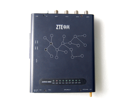
\includegraphics[width=100pt]{6600.png}

将3600的核心部分和6600主板对接.6600主板是一个linux系统,主要完成串口通信协议的制定和实现.

\subsubsection{1800 OBU(ETC高速不停车消费的车载标签)}

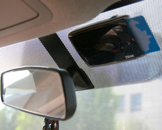
\includegraphics[width=100pt]{1800.png}

内容包括协议和驱动. 整个设备是一个MSP430的CPU裸跑,无任何操作系统. 由于要实现空中速率512kpbs, 导致要榨干CPU资源,物理层部分需要用汇编编码.难度比较大,经过长时间奋战,攻克了难关.驱动方面,完成了PSAM部分的编写. PSAM通常上讲,就是我们用的电话卡.主要是实现14443协议.经过编码实现了这个协议.

\subsubsection{8900 RSU(ETC高速不停车消费的阅读器)}
 
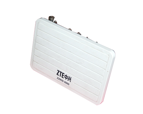
\includegraphics[width=100pt]{8900.png}

系统搭建是PPC上跑LINUX. 主要实现 PSAM在linux的驱动.由于要跑在内核态.我完成了相关驱动的编写.

\subsubsection{6602 高频发卡机}
 
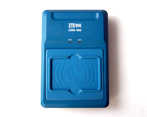
\includegraphics[width=100pt]{6602.png}

此设备是搭建在ARM7TDMI + freeRTOS + lwip 上. 我负责整体软件.并参与开发.这个设备涉及到PN531芯片的使用. 以及各种外设. 包括串口,i2c, spi, usb, eth, rs485, lcd, dac, adc等. 整个系统搭建在freertos.

\subsubsection{6205 高频发卡机}
此设备是搭建在MSP430裸跑. 我主要实现了14443B协议. 期间有一个项目在北京,比较紧急,我们在宾馆和TI工程师紧急调试完成(协议芯片是用的TI的)

\subsubsection{6602C1 RFSIM发卡机}
此设备是搭建在PPC + Linux上. 我负责整体软件. 

\subsubsection{1601 有源EPC 标签}
此设备类似3600, 用更小的资源实现标签测的功能.我完成了相应标签测的编码工作.



\subsection{研究生华为3COM实习}

研究生阶段,在华三实习,实习的平台是私有的操作系统,这个操作系统实际上是封装了vxworks和psos两个操作系统的系统调用。实际工作是维护x.25协议栈。开发atm协议的新功能。完成lapb的新功能。给泰国项目添加了LAPB的T4功能.由于时间紧迫,当初是熬夜完成了这个工作.

\subsubsection{ATM信元透传项目}
此项目由中国联通提出,要完成在MPLS L2VPN网络上对ATM信元进行透传,需要将ATM信元按照IETF的草案进行打包,透过MPLS网络进行透传。 

\subsubsection{X2T支持携带地址功能项目}
在华为3com公司进行,此项目由中国空军管理基地提出,需要完成在X2T报文中添加目的和源X.121地址的功能,用来代替博达公司的路由器。 

\subsubsection{X.25禁止流控协商项目}
在华为3com公司进行,此项目由泰国银行提出,需要完成X.25交换设备不对两侧进行流控协商,用来代替思科公司的路由器。 

\subsubsection{泰国KTB紧急项目}
在华为3com公司进行,由于“X.25禁止流控协商项目”项目分析有偏差,需要在3天的时间内完成LAPB T4功能,来不停地发送SABM。我在3天之内通宵熬夜完成了此任务。

\section{个人性格}

\begin{compactitem}
    \item 勤奋,踏实
    \item {\color{red}stay hungry, stay foolish. Be a humble man}
    \item 希望有生之年能做出{\color{red}改变大众生活习惯的创造性产品}
    \item 爱学习,读书,喜欢编程
    \item 成为技术专家是我的梦想
    \item 爱音乐(古典,流行),足球
\end{compactitem}




\section{感悟}
\subsection{有关嵌入式}
以后的世界,嵌入式设备将占有很大比例.几年前,谁能想象,安卓手机的出现?谁能想象,现在的设备nand可以达到8g?由于硬件的发展.导致嵌入式设备可以使用的资源越来越大,直接导致linux/android可以跑在很多嵌入式设备上, 资源的扩张,我们可以不拘泥于C语言, 可以用python, ruby等实现一些我们想要的功能.而另一方面,小型设备由于体积,成本的原因,也会有裸机跑程序的情况出现.

\subsection{android/ ubuntu phone}

我相信,以后开源世界,将会是这两个的天下. android 由于采用jvm, 上层套了一层java, 导致整个系统其实很庞大. 而ubuntu phone则是原生于linux, 可使用的资源很多.最根本的问题,是哲学的问题.反应在许可证上. linux是GNU/Linux, 采用的GPL,描绘了一个理想国, 一切尽开源.而android为了迎合硬件厂商,采用的apache, 驱动有些是闭源的. android是google主导的.而ubuntu是社区推动的.

\subsection{如何写文档}
对于一个技术人员.对排版的需求并不是很大, 我经历了word-markdown-LaTeX 的转变.对于markdown生成pdf,我研究了progit的代码.发现progit就是使用latex将markdown转换成pdf的. 在平常我习惯于latex.

\subsection{linux的发行版}

我经历了ubuntu-arch-gentoo-arch-gentoo. 我目前已经只用gentoo了.虽然装麻烦些. 但是其优秀的包管理工具是我选择这个发型版的原因之一.虽然这个发行版由于复杂性,注定不能普及.

\subsection{linux的界面}

曾经使用过awesome和subtle. 发现他们的bug很是耗费经历,一段时间内我使用kde,目前使用更有效率的awesome.

\subsection{文本编译器/ide}

有了{\color{red}vim},还需要其他么?

\end{document}

